\textit{Nous avons fait le choix de débuter notre travail en rédigeant un cahier des charges sommaire. Ce premier travail, réalisé en équipe, nous a permis de cerner le sujet et de lister les besoins ainsi que les contraintes imposées. Le modèle de données proposé sera également exposé. L’objectif de l'application est de permettre une visualisation de schémas relationnels de bases de données hébergées sous des serveurs de données hétérogènes.}


\section{Fonctions principales}
		\subsection{Données d'un schéma de base de données}
		La fonction principale de l'application est de fournir les données d'un schéma d'une base de données. Un schéma est composé de tables, de colonne et de contraintes. Les informations qui doivent être fournies sont décrites ci-après.
		
			\paragraph{tables}
			Une table est contenue dans un schéma (base de données)
				\begin{itemize}
					\item NAME, nom de la table
				\end{itemize}
				
			\paragraph{colonne}
			Une colonne est contenue dans une table.
				\begin{itemize}
					\item NAME, nom de la colonne
					\item TYPE, type représentant le domaine de valeur accepté
					\item PRECISION, précision du type de la colonne
				\end{itemize}
				
			\paragraph{contraintes}
			Une contrainte s'applique sur une ou plusieurs colonnes d'une table.
				\begin{itemize}
					\item NAME, nom de la contrainte
					\item TYPE, type de la contrainte
				\end{itemize} 
				
				Les contraintes suivante doivent être gérées : 
				
				\begin{itemize}
				\item Contrainte d'unicité : qui permettent d'identifier de manière unique un enregistrement dans les tables (UNIQUE, PRIMARY KEY).
				\item Contraintes référentielles : qui servent à établir des relations entre les tables (FOREIGN KEY).
				\item Contraintes de vérification de la validité des données (CHECK)
				\end{itemize}
				
		\subsection{Visualisation graphique}
		Dans le but d'assurer une représentation aisément compréhensible, l'application doit permettre la visualisation du schéma de manière graphique.

\section{Fonctions contraintes}
	\subsection{Compatibilité \& extensibilité}
	L'outil développé devra être compatible avec les SGBDR les plus populaires (\emph{Mysql}, \emph{Postgresql}, \emph{Oracle}, etc.). L'architecture de l'application devra être pensée de manière à pouvoir étendre facilement la compatibilité avec de nouveaux SGBDR en utilisant, par exmple, des fichiers de configuration. De plus, les schémas relationnels étant associés logiquement, elle devra être capable de composer de l’information provenant de l’intégration de ces différents schémas.
	\subsection{Utilisation d'Hibernate}
	L'objectif de ce projet étant l'application des outils vus pendant les cours de l'UE Gestion de données distribuées (GMIN210), l'outil développé devra utiliser l'ORM \emph{Hibernate} (librairie Java de mapping Object-Relationnel). Cette contrainte est imposée par le sujet. L'exploitation de la solution de projection Objet-Relationnel Hibernate se fera par définition des fichiers de mapping nécessaires et des classes applicatives qui permettront de manipuler les objets Table, Attribut ou Contrainte.
	\subsection{Lecture des Métadonnées}
	La lecture des métadonnées s'effectuera à partir d'une connexion à \textbf{une base de données}. Les métadonnées devront être chargées directement à partir des vues proposées par les différents SGBDR, via un connecteur. L'ORM \emph{Hibernate} étant imposé, le connecteur utilisé sera probablement \emph{JDBC}.

\section{Modélisation proposée}
\label{section:modelisation_proposee}

La figure~\ref{figure:diag_classe_fournit} présente le modèle de donnée de l'application, décrit dans le sujet. Il présente les éléments qui composent une base de données.

\begin{figure}[H]
\centering
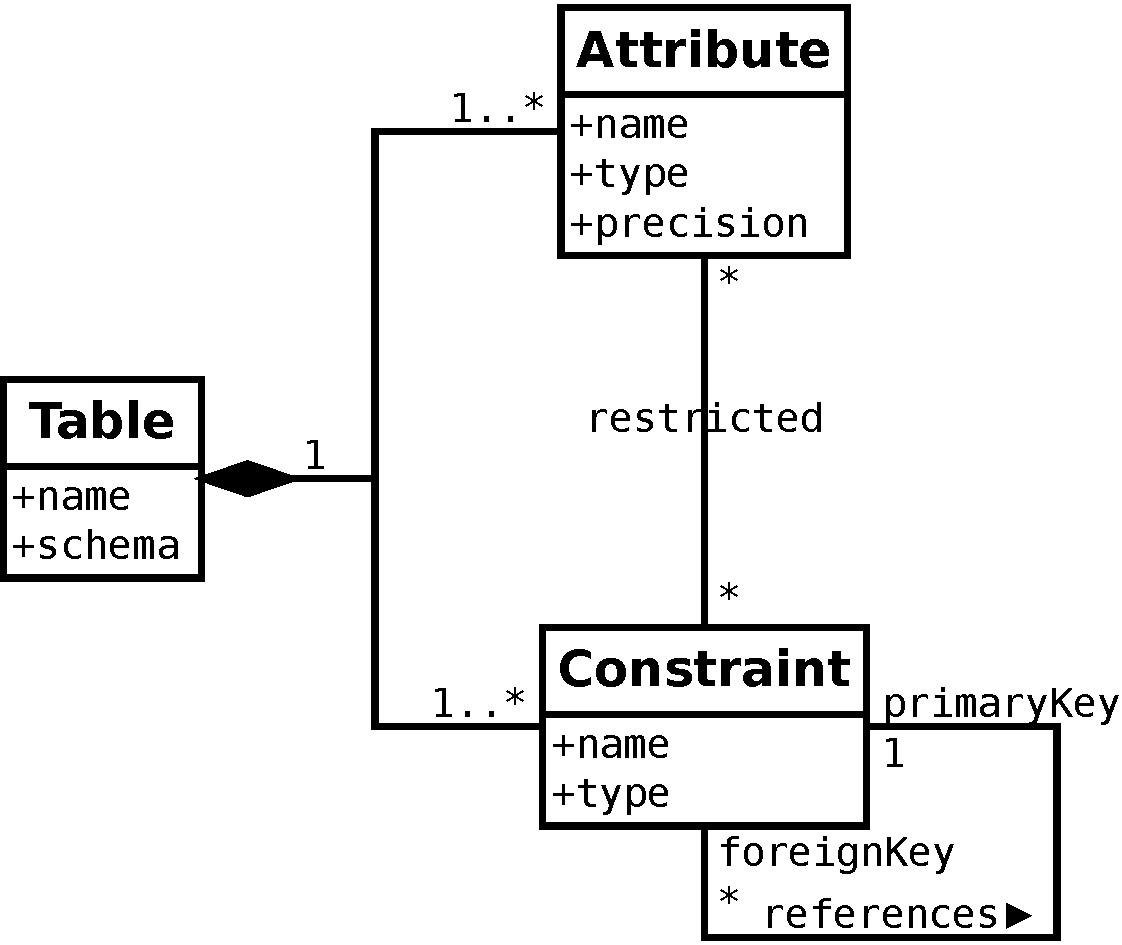
\includegraphics[width=0.6\textwidth]{files/diag_class_origine}
\caption{Diagramme de classe fournit.}
\label{figure:diag_classe_fournit}
\end{figure}

Une table est caractérisée par son nom et le nom du schéma dans lequel elle appartient. Elle est composée d'attributs et de contraintes. Un attribut, appartenant à une table, est caractérisé par son nom et son type (avec une précision). Une contrainte possède un nom et un type. Elle peut s'appliquer (restreindre) à un attribut et, dans le cas d'une clé étrangère, référencer une contrainte de clé primaire.